% LaTeX Template for Project Report,
% It is advisable to learn the basics of LaTeX before using this template.
% A good resource to start with is http://en.wikibooks.org/wiki/LaTeX/
% Empty space after chapter/section/subsection titles can be used to insert text.
%
% Just compile this file after making all required changes.

\documentclass[12pt,a4paper]{report}
\usepackage[bookmarks, colorlinks=false, pdfborder={0 0 0}, pdftitle={Book Store App}, pdfauthor={Chirag.K.Deshbhandari, Vinay Chandra}, pdfsubject={Project Report}, pdfkeywords={report}]{hyperref} %for creating links in the pdf version and other additional pdf attributes, no effect on the printed document


%adjust your page margins here
\usepackage[top=0.8in, bottom=0.75in, left=1.25in,right=1in]{geometry} % setting the page alignment with this package

%To change line spacing in a specific environment you will use the second way, which is to add \usepackage{setspace} to the preamble and then you can make use of the command \singlespacing, \doublespacing, or \onehalfspacing to specify the line spacing for all sections and paragraphs until you sued another command to change it.
\usepackage{setspace} 

%for page borders use this package
\usepackage{fancybox}

%use this package to change the default chapter number and name display
\usepackage{titlesec}

%for embedding images
\usepackage[pdftex]{graphicx} 

%for proper url entries
\usepackage{url} 

% Renewed commands to set the titles of various pages correctly.
\renewcommand\contentsname{\centering TABLE OF CONTENTS}
   \renewcommand\listfigurename{\centering LIST OF FIGURES}
   
   \renewcommand\bibname{\centering REFERENCES}
   \renewcommand\appendixname{APPENDIX}

%to display chapter number left and chapter title center
\titleformat{\chapter}[display]
  {\normalfont\Large\bfseries}{\filright\chaptertitlename\ \thechapter}
  {20pt}{\Huge\filcenter}
	
\begin{document}



\begin{titlepage}

\begin{center}
%\begin{framed}
\thispagestyle{empty}
\thisfancypage{%
  \setlength{\fboxsep}{10pt}\doublebox}{}
	
\onehalfspacing
\LARGE{\textbf{Malnad College of Engineering, Hassan}} \\
\large{
(An Autonomous Institution affiliated to VTU, Belgavi)}\\[0.2in]
\vspace{0.3cm}
%MODIFY THE LOGO/DEPARTMENT NAME/COLLEGE NAME/ADDRESS IF YOU HAVE TO, ELSE LEAVE IT

\includegraphics[width=0.18\textwidth]{./vtu_logo.jpg}\\[0.3in]

\Large{\small{A Mini Project Report \\ On}}\\
% Title
\Large{\textsc {\textbf{``Book Store App"}}}\\[0.3cm]
%Example
%\Huge{\textsc {\textbf{A case study on linux}}}\\[1.0cm]
\small \emph{Submitted in partial fulfillment of\\
        the requirements for the award of the degree of}
        \vspace{.2in}

       {\bf Bachelor of Engineering \\in\\ Computer Science and Engineering}\\[0.25cm]
\vspace{1cm}					
% Submitted by
\normalsize Submitted by \\
\begin{table}[h]
\centering
\begin{tabular}{lr}
Chirag.K.Deshbhandari & 4MC19CS035 \\
Vinay Chandra & 4MC19CS188 \\ 
\end{tabular}
\end{table}

\vspace{0.6cm}
Under the guidance of\\
{\textbf{Mr. Shashidhara H V}}\\
Associate Professor\\
\vspace{1cm}

\includegraphics[width=0.18\textwidth]{./mce_logo.png}\\[0.1in]



% Bottom of the page
%
\includegraphics[width=0.18\textwidth]{./mce_logo.png}\\[0.1in]
\Large{\bf Department of Computer Science and Engineering}\\


%\vspace{0.1cm}
\bf 2022-2023

%\end{framed}
\end{center}

\end{titlepage}

\newpage

\thispagestyle{empty}

\thisfancypage{%
  \setlength{\fboxsep}{10pt}\doublebox}{}
	
\vspace*{1\baselineskip}
\begin{center}

\LARGE{\textbf{Malnad College of Engineering}} \\ 
\large{\textbf{Department of Computer Science and Engineering}}\\
\large{\textbf{Hassan - 573201, Karnataka, India}}\\[0.5cm]


\includegraphics[scale=0.5]{mce_logo.png}\\[0.5cm]

\emph{\LARGE Certificate}\\[1cm]
\end{center}

This is to certify that mini project work entitled \textbf{``Book Store App"} is a bonafide work carried out by \textbf{Chirag.K.Deshbhandari(4MC19CS035),
Vinay Chandra (4MC19CS188)} in partial fulfillment for the award of  Bachelor of Engineering in Computer Science and Engineering of the Visvesvaraya Technological University, Belgavi during the year 2022-2023.   The project report has been approved as it satisfies the academic requirements in respect of mini project work prescribed for the Bachelor of Engineering Degree. \\[1.0cm]

\vspace{0.25cm}

\begin{table}[h]
\centering
\begin{tabular}{lllll}
Signature of the Guide & & Signature of the HOD & & Signature of the Principal \\
Mr. Shashidhara H V  & & 	Dr. Geetha Kiran A & & Dr. S. Pradeep  \\ 
Associate Professor & &  Prof. \& HOD & & Principal \\
Dept. of CSE, MCE & & Dept. of CSE, MCE & & MCE
\end{tabular}
\end{table}
\vspace{0.5cm}
\begin{center}
Examiners
\end{center}
\vspace{-0.75cm}
\begin{table}[h]
\centering
\begin{tabular}{lll}
Name of the Examiner & \hspace{4cm}  & Signature of the Examiner
\end{tabular}
\end{table}
\vspace{-0.75cm}
\begin{enumerate}
\item  \vspace{0.25cm}
\item
\end{enumerate}

\newpage
\begin{center}
\thispagestyle{empty}
\vspace*{2\baselineskip}
\LARGE{\textbf{ABSTRACT}}\\[0.5cm]
\end{center}
\thispagestyle{empty}
\doublespacing
\begin{normalsize}
Books play the most important role in our life! Books help us to give the knowledge. We can 
read a book while relaxing, leisure time and they provide good source of knowledge. Books 
are our teachers, friends and guides and philosopher also. They provide enriching experience 
and thoughts. So we called "BOOKS ARE HUMAN'S BEST FRIEND."
The app brings the power of books at your fingertips. Its combines the world of Google books 
store into one single place with a very simple, easy to understand interface.
No expert knowledge and learning curve involved.
This system is an app developed on the basis of Android. Android Studio  are used as tools to develop this. When you read a good book, you can see others and see yourself, and you can get a lot of insights every time. Reading is a very popular thing to do. No matter how busy a job is, people will spend a certain amount of time buying books and reading books. The app design page is beautiful, friendly user interface, high user experience, on the online bookstore app, buyers and bookstore managers can achieve their own needs. Book purchasers can quickly buy their favorite books. Bookstore administrators can deal with orders formed after book buyers' books in the first time and update books in bookstores in time. The development of such app is of great significance for economic development, and much more convenient for consumers to use.
\\[1cm]
\end{normalsize}
\newpage
%\vspace*{1\baselineskip}
\begin{center}
\thispagestyle{empty}
\LARGE{\textbf{ACKNOWLEDGEMENTS}}\\[1cm]
\end{center}
\vspace{0.05cm}
\doublespacing


We present with immense pleasure this work titled \textbf{”Book Store App”}. An endeavour over a long period can be successful with the advice and support of
many well wishers.


We take this opportunity to express our gratitude and appreciation
to all of them.
The satisfaction and euphoria that accompany the successful completion of any
task would be incomplete without mentioning the people who made it possible. So,
with gratitude we acknowledge all those whose guidance and encouragement made to
successfully complete this project.


We would like to express sincere thanks to our Principal \textbf{Dr. Pradeep S}, Malnad
College of Engineering for his encouragement made to successfully completion of the
project work.
We wish to express our gratitude to \textbf{Dr.Geetha Kiran A}, Professor and Head,
Department of Computer Science \& Engineering for providing a good working environment and for her constant
support and encouragement.


It gives great pleasure in placing on record a deep sense of gratitude to our guide
\textbf{Mr. Shashidhara H V},Associate Professor, Department of Computer Science \& Engineering for his daily evaluation of the work and for providing us constant encouragement with his unflinching support and valuable guidance throughout this project.

We would also like to thank all the staff of Computer Science and Engineering
department who have directly or indirectly helped us in the completion of the project
work.
At last we would hereby acknowledge and thank our parents who have been a
source of inspiration and also instrumental in the successful completion of the project
work. \\
\large{\hspace*{4.5in} Chirag.K.Deshbhandari}\\
\large{\hspace*{4.5in} Vinay Chandra}





\pagenumbering{roman} %numbering before main content starts
\tableofcontents
\listoffigures

\newpage
\pagenumbering{arabic} %reset numbering to normal for the main content

\onehalfspacing
\chapter{Introduction}

\section{Introduction}
\subsection{Introduction to BookStore}

\begin{figure}[h]\centering
	
\includegraphics[width=2in]{images.jpg}
	\caption{Books}\label{Books}
\end{figure}

 This app allow the authors and book store owners to sell and rent their books to the people who are interested in reading those particular books in return for money.

With the help of an online book store marketplace, users can simply make their accounts on this app, if they want to use and start looking up the books they are interested in.

By applying filters and entering the author name of the book they are looking for or a keyword, they get a variety of suggestions.

There, they get a lot of options to choose from and add the book they are interested in buying to the cart and make the payment.

Payment mode is cash on delivery, where the customer will get an OTP after ordering the books. The delivery boy asks the OTP from the customer and confirms the delivery at your doorstep.


\subsection{Problem Statement}
We need to understand that bookstores are not just a place to sell a product. Bookstores are
one of the most important elements of any high street – we give advice, we give directions, we
act as tour guides and we host events and help keep local communities alive. We also try to sell
them books.We are a nation known for fantastic writers and bookstores are part of our culture.
If we value this we need to support our local stores.
Bookstores are one of the most important elements of any high street – we give advice, we give
directions, we act as tour guides and we host events and help keep local communities alive. We
also try to sell them books. We are a nation known for fantastic writers and bookstores are part
of our culture


\section{About Project}
Book Store App allows users to check for various Books Instruments and can purchase them. The project consists of list of Books displayed in various models and designs. The user may browse through these products as per categories. If the user likes a product he may add it to his shopping cart. The User can view the items based on their names & Price in increasing or decreasing order.
This App has an Innovative Floating Cart that is available on each page, which pops up showing the Items that are currently in the cart with minimum details. The User must first register into the system and then is eligible to check out the products. The User has 3 kinds of payment method namely; Debit, Credit card or Cash on Delivery. The Front End of the App is done using Android Studio and SQL serves as a backend to store books lists and inventory data. The products are added by the Admin, The Admin Part uses Asp.Net with C#. Thus the online books shopping project brings an entire Books Store online and makes it easy for both buyer and seller to make deals on Books. The User can check his order history or the status of the current order in my orders column. Admin is responsible for changing the status of the orders.


•	User Registration: User has to register to check out the products and buy them.

•	User Login: User can login to system and check various Books.

•	Home: Home Page contains 5 items of each Category for the user to know the clarity of the app and items are clickable. 

•	Product Categories: The Books are arranged and can be viewed in categories.

•	Filters: Filters can be applied on the items based on their price and name in their increasing or decreasing order. By default the items are arranged in the alphabetic order.

•	Add to cart: Users can add Books to cart.

•	Floating Cart: The App gives the user a Floating Cart on every page for checking current items in the cart.

•	Credit/Debit card payment: After total bill is calculated user can pay via credit card online

•	Cash on Delivery: The Address of the user is already taken while his registration and can be updated in the My Details Page.

•	My Orders: The user can check all his order history and the status of his orders.

•	Admin: Admin adds the items and their details and changes the status of an order. 

\section{Aim, Scope and Objectives}
\subsection{Aim}
Book shopping App allows users to check for various Books Instruments and can purchase them. The project consists of list of Books displayed in various models and designs. The user may browse through these products as per categories. If the user likes a product he may add it to his/her shopping cart.
\subsection{Scope}
As a part of the preliminary study, the scope of the system has to be clearly outlined. This is useful
forestimating the amount of effort required, the cost involved etc. In any Book store Purchase and Billing
department play an important role to produce great image in market. We cannot think about an existence of an
individual department only. Here the Purchase department deals with all the procedure regarding the purchase
of the shoes from the party. Here the billing department deals with all the procedure regarding the sale of the
shoed to the client. During the purchase or billing procedure the Book store will interact with the party or with
the client as external entity and with other departments inside the environment of Book store. The boundaries of
the system is the system is the boundary of the Book store which encloses the different departments including
the purchase and sale department which interact with the external entities as Party and Client.
\subsection{Objectives}
The main objective of the Android Book Store is to manage the details of Books, Customer, Payment, Delivery, Bills. 
It manages all the information about Books, Stock, Bills, Books. 
The project is totally built at administrative end and thus only the administrator is guaranteed the access and is specially built for book store owners and authors. % adds the introduction page
\chapter{Requirements}

Generally customers go to the book store to buy a book of there likes and people come from far away places.This Book Store App makes the customers a easy means of getting the book within a few clicks by ordering the books from there homes

\section{Hardware Requirements(PC)}
\begin{itemize}
\item Microsoft® Windows® 8/10 (32 or 64-bit)
\item 2 GB RAM minimum, 4 GB RAM recommended
\item 400 MB hard disk space At least 1 GB for Android SDK (software development kit)
\item emulator system images, and caches 1280 x 800 minimum screen resolution.
\item Java Development Kit (JDK) 8.
\end{itemize}

\section{Software Requirements}
\begin{center}
\begin{itemize}
    \item In Android Studio - Android SDK, 
       debugging tools, 
       emulators, 
       graphical UI builder. 
       Database: MySQL
\item Xml for layouts
        
\end{itemize}
\end{center}

\chapter{Project Design}
\section{System Design}
The flow chart shown in Fig. \ref{design} is the system design representing interfaces and functional flow of the Book Store App android based project.

\begin{figure}[h]\centering
	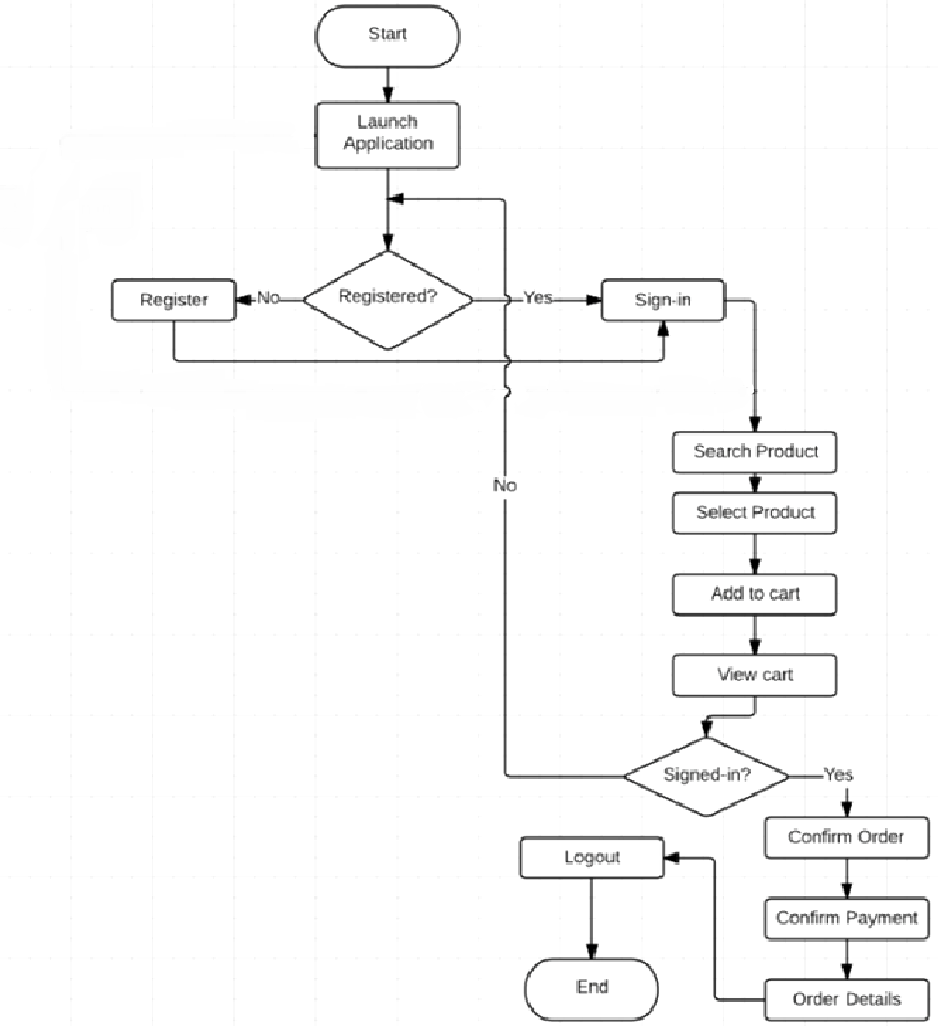
\includegraphics[width=4.8in]{design.png}
	\caption{System design of Book Store App}\label{design}
\end{figure}
 % adds the Project Design
\chapter{Implementation}
\section{Methodology}
This android application is implemented using the technologies such as basic android studio involving Java ,XML and json. Also, we have used few modules required to implement the otp generation for the confirmation of product delivery by the delivery boy at the customers doorsteps . 
\begin{itemize}
    \item Registration: Customer can register their account here to continue shopping.
    \item Admin: Admin can add books, check orders and make sure the orders are delivered on time and can confirm payments by the customers.
    \item Shopping Cart: Customers after login can browse through the different books and choose one or more products and can add them to cart
    \item Payment: Cash on Delivery facility is available

\end{itemize}





 % adds the implementation
\chapter{Result of Book Store App }

\section{Output}

\subsection{Login page for both customer or seller}

\begin{figure}[h]\centering
	\includegraphics[width=3in]{./images/login.png}
	\caption{User Login as Customer or Seller}\label{login}
\end{figure}



\begin{figure}[h]\centering
	\includegraphics[width=1.9in]{./images/User Profile.png}
	\caption{User Profile}\label{profile}
\end{figure}

\pagebreak

\subsection{Book List and Search}
\begin{figure}[h]\centering
	\includegraphics[width=1.9in]{./images/Books list with fixed rate.png}
	\caption{List of Books with a fixed rate}\label{Book list}
\end{figure}

\begin{figure}[h]\centering
	\includegraphics[width=1.9in]{./images/Search Book.png}
	\caption{To search the exact name of the book}\label{search book}
\end{figure}

\pagebreak

\subsection{Buy ,Rent Book and OTP generation}
\begin{figure}[h]\centering
	\includegraphics[width=1.9in]{./images/Buy Book.png}
	\caption{Buy a Book with a fixed rate}\label{Buy Book}
\end{figure}

\begin{figure}[h]\centering
	\includegraphics[width=1.9in]{./images/Rent Book.png}
	\caption{To rent the book for some days, weeks or even months}\label{rent book}
\end{figure}

\pagebreak

\begin{figure}[h]\centering
	\includegraphics[width=1.9in]{./images/Payment and OTP.png}
	\caption{Delivery boy recieves the otp from the customer and confirms delivery}\label{OTP generation}
\end{figure}

\subsection{Seller side}

\begin{figure}[h]\centering
	\includegraphics[width=1.9in]{./images/seller dashboard.png}
	\caption{Dashboard of Seller}\label{seller dashboard}
\end{figure}

\begin{figure}[h]\centering
	\includegraphics[width=1.9in]{./images/Add Book for Seller.png}
	\caption{To add book with amount and delivery charges}\label{add book}
\end{figure}

\pagebreak

% \begin{figure}[h]\centering
%     \includegraphics[width=6in]{./images/invoiceorder.jpg}
% 	\caption{Print the invoice from generated invoice PDF}\label{invoiceorder}
% 	\includegraphics[width=6in]{./images/invoiceorderitem.jpg}
% 	\caption{Print the invoice from generated invoice PDF}\label{invoiceorderitem}
% 	\includegraphics[width=6in]{./images/invoiceuser.jpg}
% 	\caption{Print the invoice from generated invoice PDF}\label{invoiceuser}
% \end{figure}
% \caption{Comparison of Community Detection Algorithms}\label{comp}				% adds result page
\chapter{Conclusion and Future Works}

\section{Conclusion}
In this Book Store project, we understood how to create a online shopping related application
with a beautiful UI design using Android Java. We can customize this project and add as many
books to improve the number of customers for our app. This app is very useful for book lovers
as there is no need to go for book shop physically but now books are avaialable to buy online


\section{Future Works}
Though our project has been completed but still betterment is always an open door. In this
case also we can improve it by: 

\begin{itemize}
\item Making the user-interface more interactive. 
\item Adding more graphical user interface
\item We can integrate our application with various book stalls so that all are available under one roof.
\item We can add text-to-speech and speech-to-text feature in our app to make it more accessible for people with disadvantages and for normal users. 
\end{itemize}
 % adds conclusion page

\pagebreak
% Appendices.
 \appendix
\chapter{Brief explanation regarding Book Store App}\label{code}
\begin{normalsize}
People today are more inclined towards online purchase, from booking tickets for flights to purchase groceries online, our lives are majorly dependent on mobile apps. When it comes to buying books, there is no exception.The online bookstore apps give authors and bookstore vendors a platform to sell or rent books to the people who love to read in exchange for some specific amount of money. Through the online bookstore marketplace, a community of readers can easily browse their favorite books, authors, genres, etc., by making an account on the app.
In the past year, the market share of online bookstores has grown exponentially. Bookstore mobile apps have generated higher revenue during this time, and it all happens because of the outbreak of the pandemic. The covid-19 situation made people ponder on their reading habits and to start with the book which they always wanted to read.
According to a survey, the global online book services market size was estimated at 17.7 billion USD in 2019, and the numbers are expected to grow at a CAGR of 5.8% from 2020 to 2027. 
By the year 2027, the global online book service market is expected to earn 27.8 billion USD as revenue.It is also believed that around 12000 people go online book shopping in a day.To leverage the huge numbers, we can plan a book store mobile app that not only can give our business great exposure but also connect our brand with potential customers easily.Amazon has revolutionized the way of selling and purchasing books. Today, people from any part of the world can read a book of their choice, published and printed in different parts of the country. The community of book readers is large, and one must have a suitable online book store mobile application to cater to the diverse book requirements of readers.In the current situation of the pandemic, the physical book stores which were flooded with people are now empty. Amidst this, having a suitable mobile application will be a perfect choice.

\\[1cm]
\end{normalsize}
 

\pagebreak
\addcontentsline{toc}{chapter}{References}
\newpage
\begin{center}
\thispagestyle{empty}
\vspace*{2\baselineskip}
\LARGE{\textbf{References}}\\[1cm]
\end{center}
\thispagestyle{empty}
\doublespacing
(1) Google Developer Training, "Android Developer Fundamentals Course – Concept 
    Reference”, Google Developer Training Team, 2017 \
 
(2) https://www.geeksforgeeks.org/android/app
 
(3) https://developer.android.com/ 
 
(4) https://www.quora.com/What-are-the-features-of-the-best-online-bookstore. 
 
(5) https://www.coursera.org/learn/java-for-android
 
(6) Akshay V,Anish Kumar S,“ BOOKAZOR - an Android Appointment Booking System”

(6) Mingxi Zhang, Chao Song, “A Framework for Discovering Similar Products from 
    Android Bookstore” 

(7) Takashi OKAMOTO, “The Study on Consumer Behavior of Android Book shops
\end{document}
